%!TEX program = xelatex
\documentclass[a4paper,10pt,twocolumn,oneside]{article}
\setlength{\columnsep}{10pt}                                                                    %兩欄模式的間距
\setlength{\columnseprule}{0pt}                                                                %兩欄模式間格線粗細

\usepackage{amsthm}								  %定義,例題
\usepackage{amssymb}
%\usepackage[margin=2cm]{geometry}
\usepackage{fontspec}								%設定字體
\usepackage{color}
\usepackage[x11names]{xcolor}
\usepackage{listings}								%顯示code用的
%\usepackage[Glenn]{fncychap}				%排版,頁面模板
\usepackage{fancyhdr}								%設定頁首頁尾
\usepackage{graphicx}								%Graphic
\usepackage{enumerate}
\usepackage{changepage}
\usepackage[compact]{titlesec}      %compact mode for reducing margin
\usepackage{amsmath}
\usepackage[CheckSingle, CJKmath]{xeCJK}
\usepackage{hyperref}
\hypersetup{
  linktoc=all,
  hidelinks
}
% \usepackage{CJKulem}

%\usepackage[T1]{fontenc}
\usepackage{courier}
\topmargin=-1pt
\headsep=5pt
\textheight=780pt
\footskip=0pt
\voffset=-40pt
\textwidth=545pt
\marginparsep=0pt
\marginparwidth=0pt
\marginparpush=0pt
\oddsidemargin=0pt
\evensidemargin=0pt
\hoffset=-42pt

%\renewcommand\listfigurename{圖目錄}
%\renewcommand\listtablename{表目錄} 

%%%%%%%%%%%%%%%%%%%%%%%%%%%%%

% 英文主字型
\setmainfont[
  Path = ./fonts/PingFang/,
  UprightFont    = *-Regular.otf,
  BoldFont       = *-Semibold.otf, % PingFang 沒有叫 Bold,而是 Semibold
  ItalicFont     = *-Light.otf,    % 沒有真的 italic,可視需要換別種
  BoldItalicFont = *-Medium.otf
]{PingFangTC}

% 等寬字型(Code 用)
\setmonofont[
  Path = ./fonts/FiraCode/,
  Ligatures = TeX
]{FiraCode}

% 中文主字型
\setCJKmainfont[
  Path = ./fonts/PingFang/,
  UprightFont    = *-Regular.otf,
  BoldFont       = *-Semibold.otf,
  ItalicFont     = *-Light.otf,
  BoldItalicFont = *-Medium.otf
]{PingFangTC}

\XeTeXlinebreaklocale "zh"						%中文自動換行
\XeTeXlinebreakskip = 0pt plus 0pt		%設定段落之間的距離
\setcounter{secnumdepth}{3}						%目錄顯示第三層

%%%%%%%%%%%%%%%%%%%%%%%%%%%%%
\makeatletter
\lst@CCPutMacro\lst@ProcessOther {"2D}{\lst@ttfamily{-{}}{-{}}}
\@empty\z@\@empty
\makeatother
\lstset{											     % Code顯示
language=C++,										   % the language of the code
basicstyle=\scriptsize\ttfamily, 	 % the size of the fonts that are used for the code
%numbers=left,										 % where to put the line-numbers
numberstyle=\footnotesize,				 % the size of the fonts that are used for the line-numbers
stepnumber=1,										   % the step between two line-numbers. If it's 1, each line  will be numbered
numbersep=5pt,										 % how far the line-numbers are from the code
backgroundcolor=\color{white},     % choose the background color. You must add \usepackage{color}
showspaces=false,									 % show spaces adding particular underscores
showstringspaces=false,						 % underline spaces within strings
showtabs=false,									   % show tabs within strings adding particular underscores
frame=false,											 % adds a frame around the code
tabsize=2,											   % sets default tabsize to 2 spaces
captionpos=b,										   % sets the caption-position to bottom
breaklines=true,									 % sets automatic line breaking
breakatwhitespace=false,					 % sets if automatic breaks should only happen at whitespace
escapeinside={\%*}{*)},						 % if you want to add a comment within your code
morekeywords={*},									 % if you want to add more keywords to the set
keywordstyle=\bfseries\color{Blue1},
commentstyle=\itshape\color{Red4},
stringstyle=\itshape\color{Green4},
literate={\ \ }{{\ }}1
}

%%%%%%%%%%%%%%%%%%%%%%%%%%%%%

\def\footnotesize{\fontsize{8}{9.5}\selectfont}
\titlespacing*{\section} {0pt}{2ex plus 1ex minus .2ex}{0.8ex plus .2ex}  % minimize margin
\titlespacing*{\subsection} {0pt}{1.75ex plus 1ex minus .2ex}{0ex plus .2ex} % minimize margin

\begin{document}
\pagestyle{fancy}
\fancyfoot{}
\fancyhead[L]{National Yang Ming Chiao Tung University - MutedByPEPPA}
\fancyhead[R]{\thepage}
\renewcommand{\headrulewidth}{0.4pt}
\renewcommand{\contentsname}{Contents} 

\scriptsize
\vspace{-2em}
\tableofcontents
\vspace{-1em}

%%%%%%%%%%%%%%%%%%%%%%%%%%%%%


\newcommand{\includecode}[2]{
  \subsection{#1}
  \vspace{-0.8em}
  \lstinputlisting{#2}
  \vspace{-1.2em}
}

\newcommand{\includetex}[2]{
  \subsection{#1}
  \input{#2}
  \vspace{-1.2em}
}

\newcommand{\sectiontitle}[1]{
  \section{#1}
  \vspace{-0.5em}
}


%%%%%%%%%%%%%%%%%%%%%%%%%%%%%

\sectiontitle{Basic}
\includecode{createFile}{../code/Basic/createFile}
\includecode{run}{../code/Basic/run}
\includecode{tem}{../code/Basic/tem.cpp}
\includecode{debug}{../code/Basic/debug.cpp}
\includecode{run.bat}{../code/Basic/run.bat}
\includecode{random}{../code/Basic/random.cpp}
\includecode{TempleHash}{../code/Basic/TempleHash.sh}

\sectiontitle{Misc}
\includecode{FastIO}{../code/Misc/FastIO.cpp}
\includecode{stress.sh}{../code/Misc/stress.sh}
\includecode{stress.bat}{../code/Misc/stress.bat}
\includecode{Timer}{../code/Misc/Timer.cpp}
\includecode{MinPlusConvolution}{../code/Misc/Min_Plus_Convolution.cpp}
\includecode{PyTrick}{../code/Misc/PyTrick.py}

\sectiontitle{Data Structure}
\includecode{Fenwick Tree}{../code/DataStructure/FenwickTree.cpp}
\includecode{Li Chao}{../code/DataStructure/LiChao.cpp}
\includecode{PBDS}{../code/DataStructure/PBDS.cpp}
\includecode{ODT}{../code/DataStructure/ODT.cpp}
\includecode{Sparse Table}{../code/DataStructure/SparseTable.cpp}
\includecode{Splay}{../code/DataStructure/SplayTree.cpp}
\includecode{Treap}{../code/DataStructure/Treap.cpp}

\sectiontitle{Matching and Flow}
\includecode{Dinic}{../code/Flow/Dinic.cpp}
\includecode{General Matching}{../code/Flow/GeneralMatching.cpp}
\includecode{KM}{../code/Flow/KM.cpp}
\includecode{MCMF}{../code/Flow/MCMF.cpp}
\includetex{Model}{../code/Flow/Model.tex}

\sectiontitle{Geometry}
\includecode{Point}{../code/Geometry/Point.cpp}
\includecode{Line}{../code/Geometry/Line.cpp}
\includecode{Circle}{../code/Geometry/Circle.cpp}
\includecode{Point to Segment Distance}{../code/Geometry/PointToSegmentDistance.cpp}
\includecode{Point In Polygon}{../code/Geometry/PointInPoly.cpp}
\includecode{Intersection of Line}{../code/Geometry/IntersectionOfLine.cpp}
\includecode{Intersection of Circles}{../code/Geometry/IntersectionOfCircles.cpp}
\includecode{Intersection of Circle and Line}{../code/Geometry/IntersectionOfCircleLine.cpp}
\includecode{Area of Circle Polygon}{../code/Geometry/AreaOfCirclePolygon.cpp}
\includecode{Convex Hull}{../code/Geometry/ConvexHull.cpp}
\includecode{Convex Trick}{../code/Geometry/ConvexTrick.cpp}
\includecode{Half Plane Intersection}{../code/Geometry/HalfPlaneIntersection.cpp}
\includecode{Minimal Enclosing Circle}{../code/Geometry/MinimalEnclosingCircle.cpp}
\includecode{Minkowski}{../code/Geometry/Minkowski.cpp}
\includecode{Point In Circumcircle}{../code/Geometry/PointInCircumcircle.cpp}
\includecode{Tangent Lines of Circle and Point}{../code/Geometry/TangentLinesOfCirclePoint.cpp}
\includecode{Tangent Lines of Circles}{../code/Geometry/TangentLinesOfCircles.cpp}
\includecode{Triangle Center}{../code/Geometry/TriangleCenter.cpp}
\includecode{Union of Circles}{../code/Geometry/UnionOfCircles.cpp}

\sectiontitle{Graph}
\includecode{Block Cut Tree}{../code/Graph/BlockCutTree.cpp}
\includecode{Count Cycles}{../code/Graph/CountCycles.cpp}
\includecode{Dominator Tree}{../code/Graph/DominatorTree.cpp}
\includecode{Enumerate Planar Face}{../code/Graph/EnumeratePlanarFace.cpp}
\includecode{Manhattan MST}{../code/Graph/ManhattanMST.cpp}
\includecode{Matroid Intersection}{../code/Graph/MatroidIntersection.cpp}
\includecode{Maximum Clique}{../code/Graph/MaxClique.cpp}
\includecode{Tree Hash}{../code/Graph/TreeHash.cpp}
\includecode{Two-SAT}{../code/Graph/TwoSAT.cpp}
\includecode{Virtual Tree}{../code/Graph/VirtualTree.cpp}

\sectiontitle{Math}
\includecode{Combinatoric}{../code/Math/Combinatoric.cpp}
\includecode{Discrete Log}{../code/Math/DiscreteLog.cpp}
\includecode{Div Floor Ceil}{../code/Math/DivFloorCeil.cpp}
\includecode{exCRT}{../code/Math/exCRT.cpp}
\includecode{Factorization}{../code/Math/Factorization.cpp}
\includecode{Floor Sum}{../code/Math/FloorSum.cpp}
\includecode{FWT}{../code/Math/FWT.cpp}
\includecode{Gauss Elimination}{../code/Math/GaussElimination.cpp}
\includecode{Lagrange Interpolation}{../code/Math/LagrageInterpolation.cpp}
\includecode{Linear Sieve}{../code/Math/LinearSieve.cpp}
\includecode{Lucas}{../code/Math/Lucas.cpp}
\includecode{Mod Int}{../code/Math/ModInt.cpp}
\includecode{Primitive Root}{../code/Math/PrimitiveRoot.cpp}
\includecode{Simplex}{../code/Math/Simplex.cpp}
\includecode{Sqrt Mod}{../code/Math/SqrtMod.cpp}
\includecode{PiCount}{../code/Math/PiCount.cpp}
\includecode{ModMin}{../code/Math/ModMin.cpp}
\includecode{FFT}{../code/Math/FFT.cpp}
\includetex{NTT prime}{../code/Math/NTTprime.tex}
\includecode{Polynomial}{../code/Math/Polynomial.cpp}
\includetex{Theorem}{../code/Math/Theorem.tex}

\sectiontitle{Stringology}
\includecode{Aho-Corasick AM}{../code/String/AhoCorasickAM.cpp}
\includecode{Double String}{../code/String/DoubleString.cpp}
\includecode{Lyndon Factorization}{../code/String/LyndonFactorization.cpp}
\includecode{Manacher}{../code/String/Manacher.cpp}
\includecode{SA-IS}{../code/String/SAIS.cpp}
\includecode{Suffix Array}{../code/String/SuffixArray.cpp}
\includecode{Z-value}{../code/String/Zvalue.cpp}

\sectiontitle{Peppa}
\includecode{LinearSolve}{../code/Math/LinearSol.cpp}
\includecode{LinearSolve}{../code/Math/NTT.cpp}
\includecode{FractionSearch}{../code?Misc/FractionSearch.cpp}

% \clearpage
% 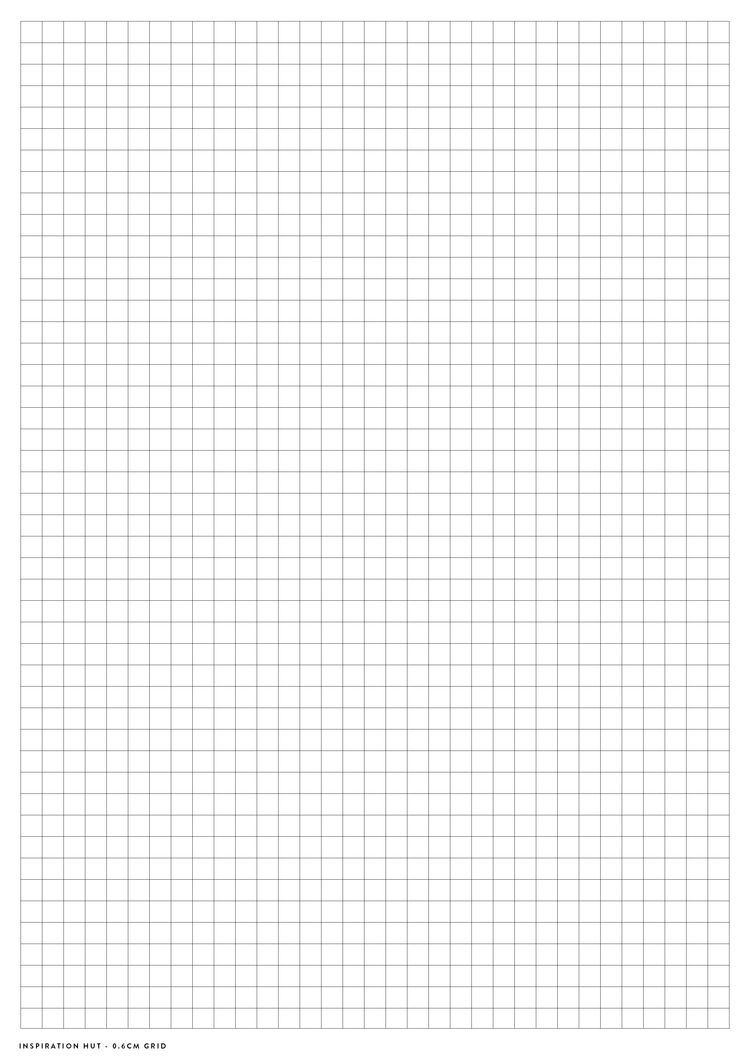
\includegraphics[scale=0.7]{grid.jpg}

% \clearpage
% 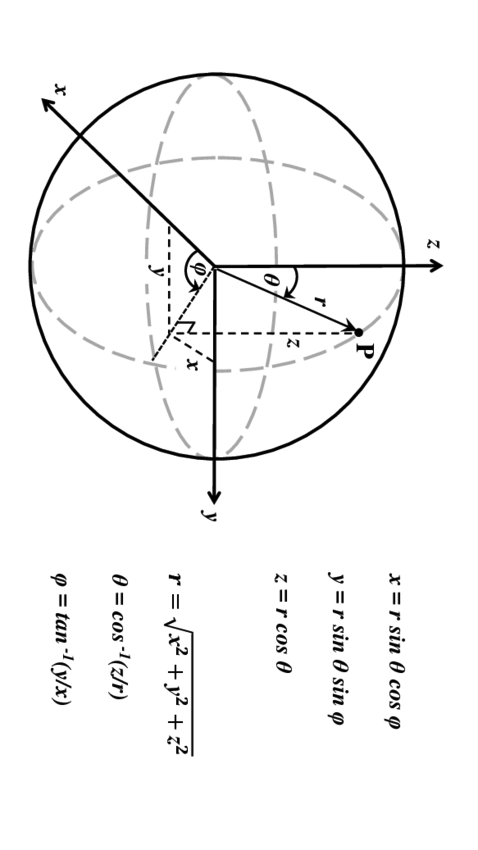
\includegraphics[scale=0.9]{Spherical-coordinates.png}

\end{document}
